\documentclass[11pt]{article}

% ====================================================
% PACKAGES
% ====================================================
\usepackage[margin=0.85in, headheight=13.6pt]{geometry}
\usepackage[T1]{fontenc}
\usepackage{lmodern}
\usepackage{microtype}
\usepackage{setspace}
\usepackage{tcolorbox}
\usepackage{amsmath, amssymb, mathtools}
\usepackage{siunitx}

\usepackage{graphicx}
\usepackage{float}
\usepackage{subcaption}
\usepackage{wrapfig}

\usepackage{enumitem}
\usepackage{booktabs}
\usepackage{array}
\usepackage{multirow}

\usepackage{xcolor}
\usepackage{hyperref}

\usepackage{fancyhdr}
\usepackage{lastpage}
\usepackage{indentfirst}
\usepackage[justification=centering]{caption}
\usepackage{listings}

\lstdefinestyle{pystyle}{
    language=Python,
    basicstyle=\ttfamily\small,
    keywordstyle=\color{blue!50!black},
    commentstyle=\color{green!40!black},
    stringstyle=\color{orange!60!black},
    numbers=left,
    numberstyle=\tiny\color{gray},
    stepnumber=1,
    numbersep=8pt,
    frame=single,
    rulecolor=\color{gray!50},
    breaklines=true,
    showstringspaces=false,
    tabsize=4
}
\lstset{style=pystyle}

\pagestyle{fancy}
\fancyhf{}
\lhead{\Assignment\ |\ \course}
\rhead{\Name\ |\ \today}
\cfoot{Page \thepage\ of~\pageref{LastPage}}

\hypersetup{
    colorlinks,
    linkcolor={red!50!black},
    citecolor={blue!50!black},
    urlcolor={blue!80!black}
}

\newcommand{\Name}{Arael Anaya}
\newcommand{\Assignment}{Final Project}
\newcommand{\course}{Advanced Dynamics (MEGN505)}

% Boxed final-answer environment (matches homework/update style)
\newtcolorbox{result}{
    colback=blue!3!white,
    colframe=blue!40!black,
    boxrule=0.6pt,
    arc=2pt,
    left=6pt, right=6pt, top=4pt, bottom=4pt
}

% Highlighted note box
\newtcolorbox{noteBox}{
    colback=blue!3!white,
    colframe=blue!40!black,
    boxrule=0.6pt,
    arc=2pt,
    left=6pt, right=6pt, top=4pt, bottom=4pt
}

% Placeholder box for work not yet completed -- flagged clearly for later passes
\newtcolorbox{insertBox}[1]{
    colback=red!4!white,
    colframe=red!55!black,
    boxrule=0.7pt,
    arc=2pt,
    left=6pt, right=6pt, top=5pt, bottom=5pt,
    title={\textbf{[INSERT HERE --- #1]}},
    fonttitle=\small\bfseries,
    coltitle=red!55!black,
}

\setlength{\parskip}{0pt}
\setlength{\parindent}{1.5em}

\begin{document}

% ====================================================
% TITLE
% ====================================================
\begin{center}
    {\Large \textbf{Dynamics and Stability of the Spring-Loaded Inverted
    Pendulum (SLIP) Model}}\\[2pt]
\end{center}
\vspace{-4pt}

% ====================================================
% 1. INTRODUCTION AND RELEVANCE
% ====================================================
\section{Introduction and Relevance}

The spring-loaded inverted pendulum (SLIP) is the reduced-order model
behind most legged-robot dynamics \cite{full1999,saranli2001}: a point
mass bouncing on a massless spring leg. Despite its simplicity, it
captures the center-of-mass dynamics of running in animals and
machines remarkably well \cite{blickhan1989,mcmahon1990}. That makes it
a good subject for this course: simple enough to analyze fully with
the tools we covered, but rich enough to produce interesting hybrid
dynamics, and it builds directly on the elastic pendulum studied in
class, since the stance phase of SLIP is an inverted spring pendulum.

SLIP is mechanically interesting as a hybrid dynamical system: during
stance the body behaves like a spring-loaded pendulum, while in flight
it is a free projectile, with the two phases connected by touchdown
and liftoff switching conditions. For a hopping gait, the natural
stability question is not about a fixed equilibrium but about whether
the periodic motion itself is stable. The standard tool for that is
the apex return map, a Poincar\'e map in which a steady hopping gait
appears as a fixed point whose stability can be assessed numerically
\cite{blickhan1989,schwind2000}.

Beyond being a convenient system, SLIP-type models are used directly
in the design and control of running robots and in the biomechanical
study of animal and human locomotion -- my practical motivation for
this project: a model simple enough to analyze by hand but predictive
enough to inform how a real legged system should be built or
controlled.

\subsection*{Relation to Prior Work}
This project works within an established line of SLIP research;
each stage of the model draws on a different part of that literature.
Blickhan \cite{blickhan1989} introduced the spring-mass template and
showed it reproduces the ground-reaction-force and center-of-mass
patterns of human and animal running; the stance-phase Lagrangian
derived here reproduces the same model, but from Lagrange's equations
in polar coordinates rather than Blickhan's Newtonian force balance.
McMahon and Cheng \cite{mcmahon1990} used the same template to relate
leg stiffness to running speed empirically; the parameter sweep over
stiffness $k$ and touchdown angle $\theta_{TD}$ planned here asks the
same question numerically, from the model directly, rather than from
experimental data. Full and Koditschek's templates-and-anchors
framework \cite{full1999} justifies treating SLIP as a legitimate
object of study on its own, not just a shortcut toward a fully
articulated multi-link leg model: a template is expected to capture
the essential dynamics of the anchored system while discarding detail
that does not matter for stability. Schwind and Koditschek
\cite{schwind2000} derived an approximate, closed-form stance map
using a perturbative solution; this project instead integrates the
stance-phase equations numerically with an event-based solver, trading
their analytical insight for an exact (if less interpretable) stance
map, consistent with this course's computational emphasis. Saranli,
Buehler, and Koditschek \cite{saranli2001} built RHex, a hexapod whose
legs behave like a SLIP template during stance -- the practical
grounding for why this abstraction is worth studying: not just a toy
system, but the model actually used to understand a working robot.
Finally, Geyer, Seyfarth, and Blickhan \cite{geyer2006} extended a
SLIP-type compliant-leg model to walking, not just running, by allowing
double support -- a natural direction for future work beyond the
single-support hopping model considered here.

% ====================================================
% 2. MODELING OF DYNAMICS
% ====================================================
\section{Modeling of Dynamics}

The equations of motion for both phases are derived using
\textbf{Lagrange's equations of motion}, with generalized coordinates
chosen separately per phase: Cartesian coordinates $(x,y)$ for flight,
and polar coordinates $(r,\theta)$ about the planted foot for stance.
The two phases are connected by touchdown and liftoff switching
(transversality) conditions, so the overall model is a hybrid
dynamical system integrated with event-based numerical methods.
Figure~\ref{fig:progress} shows the geometry of both phases.

\begin{figure}[H]
    \centering
    \vspace{-4pt}
    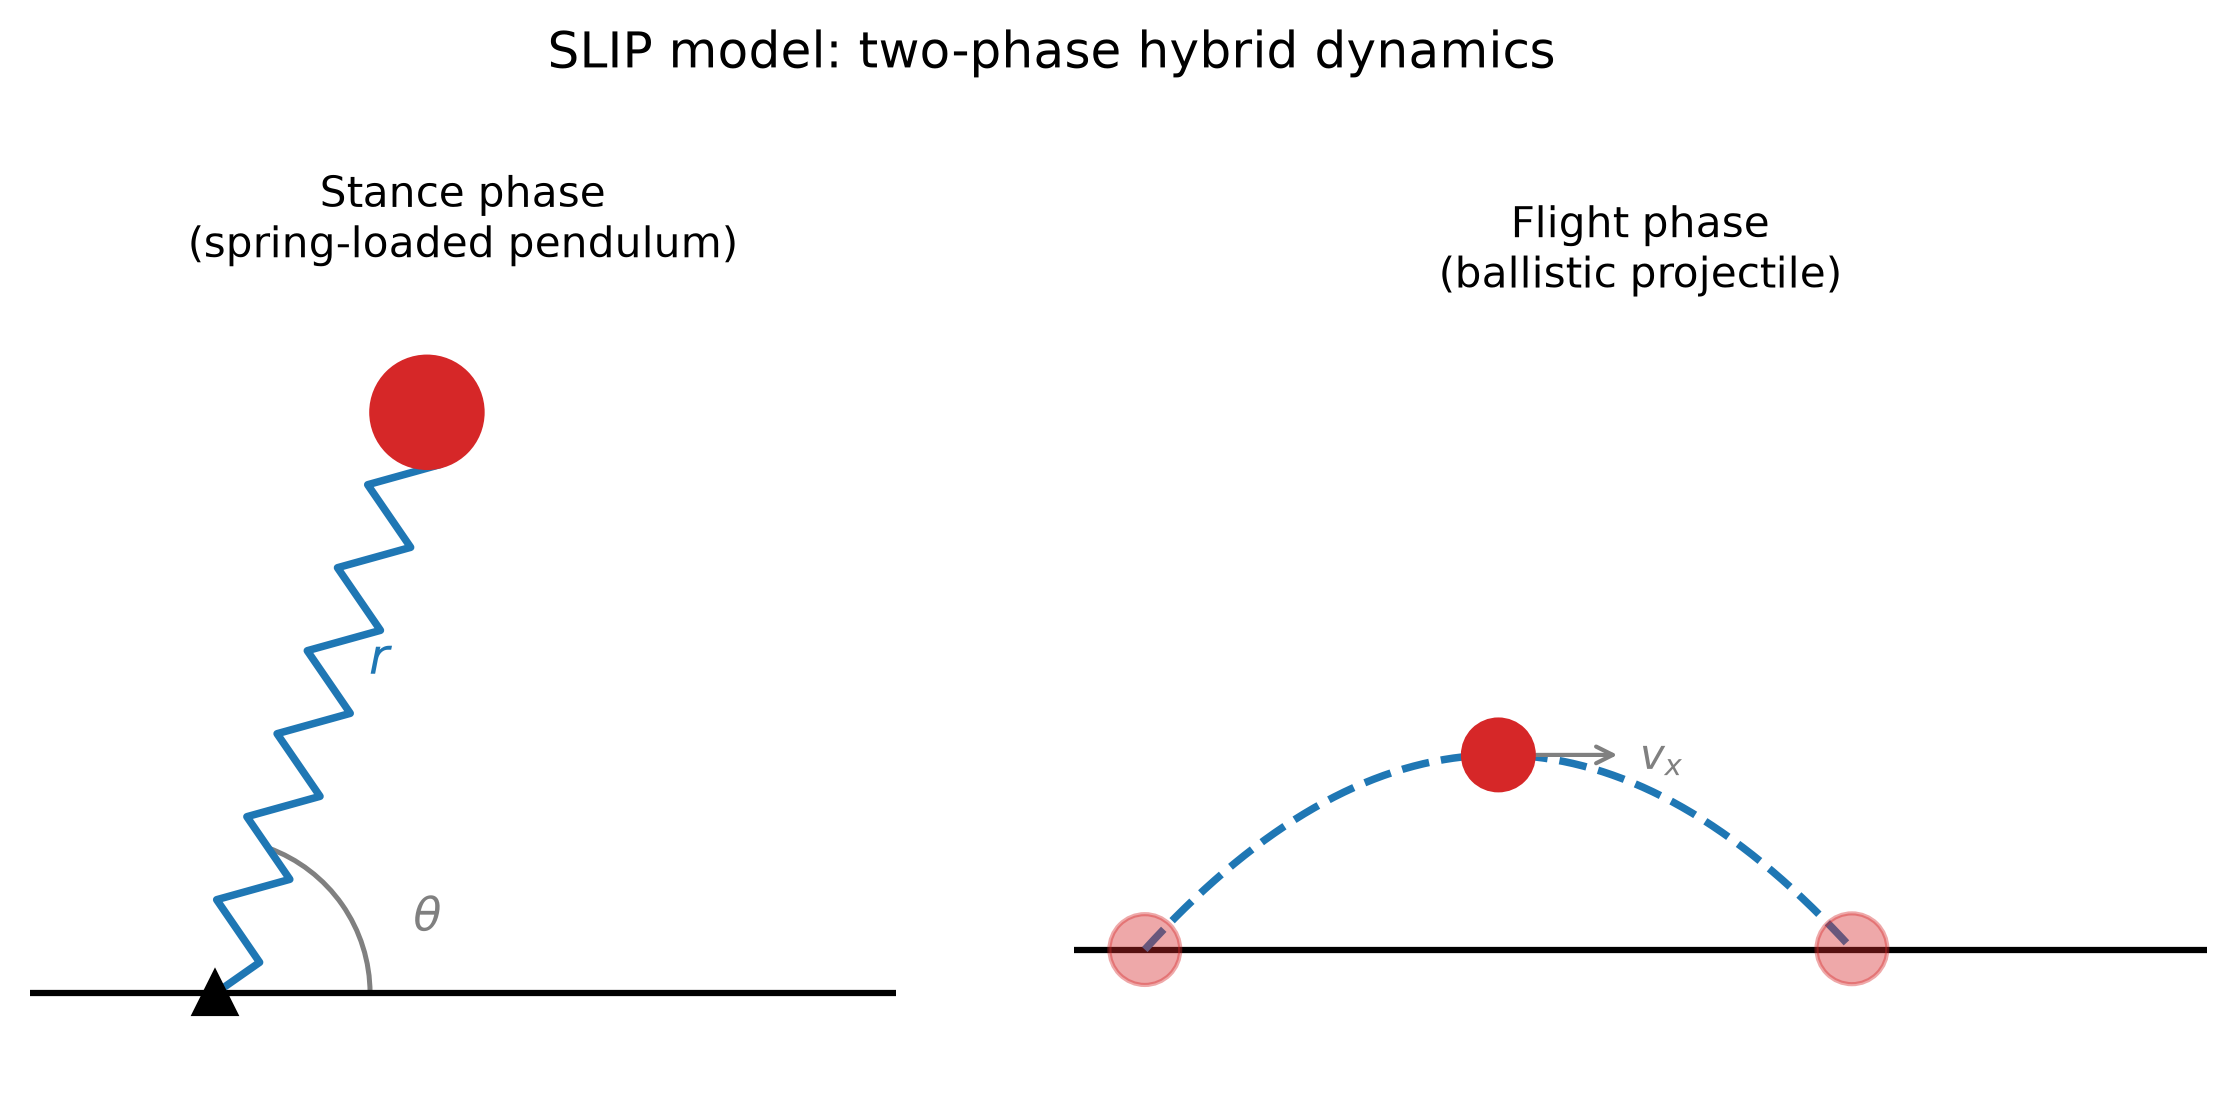
\includegraphics[width=0.55\linewidth]{Figures/progress_figure.png}
    \vspace{-6pt}
    \caption{\footnotesize SLIP model geometry: stance (spring pendulum,
    $r,\theta$) and flight (projectile).}
    \label{fig:progress}
\end{figure}

\subsection{Flight-Phase Equations of Motion}
With basis $\hat n_1,\hat n_2$, $\vec r_m=x\hat n_1+y\hat n_2$:
\[
    T=\frac12 m(\dot x^2+\dot y^2), \qquad V=mgy, \qquad
    L=T-V=\frac12m(\dot x^2+\dot y^2)-mgy
\]
Lagrange's equations give
\begin{result}
\[
    \ddot x = 0, \qquad \ddot y = -g
\]
\end{result}
Starting at the apex ($\dot y=0$), with $x(0)=x_0$, $\dot x(0)=v_{x0}$:
\[
    x(t)=v_{x0}t+x_0, \qquad y(t)=y_0-\frac{g}{2}t^2
\]

\subsection{Touchdown: Detection and Transition Map}
$\theta_{TD}$ is held fixed in flight, so the foot trails the body at
\[
    \vec r_{foot}(t) = \big(x(t)-r_0\cos\theta_{TD}\big)\hat n_1
    + \big(y(t)-r_0\sin\theta_{TD}\big)\hat n_2
\]
Touchdown is $y_{foot}=0$, i.e. $y_{TD}=r_0\sin\theta_{TD}$. Solving
$y(t)=y_0-\tfrac g2t^2$:
\begin{result}
\[
    t_{TD}=\sqrt{\frac{2(y_0-r_0\sin\theta_{TD})}{g}}, \qquad
    \dot y_{TD}=-\sqrt{2g(y_0-r_0\sin\theta_{TD})}, \qquad
    x_{TD}=v_{x0}t_{TD}, \qquad \dot x_{TD}=v_{x0}
\]
\end{result}
Stance uses polar coordinates about the planted foot, so this Cartesian
state must be converted. With foot at
$\vec r_F=(x_{TD}+r_0\cos\theta_{TD})\hat n_1$ and leg vector
$\vec\rho=\vec r_m-\vec r_F=-r_0\cos\theta_{TD}\,\hat n_1+y_{TD}\hat n_2$:
\[
    r = |\vec\rho| = \sqrt{r_0^2\cos^2\theta_{TD}+y_{TD}^2} = r_0, \qquad
    \theta = \operatorname{atan2}\!\big(y_{TD},\,-r_0\cos\theta_{TD}\big)
\]
Projecting $\vec v=\dot x_{TD}\hat n_1+\dot y_{TD}\hat n_2$ onto
$\hat e_r=\cos\theta\,\hat n_1+\sin\theta\,\hat n_2$,
$\hat e_\theta=-\sin\theta\,\hat n_1+\cos\theta\,\hat n_2$:
\begin{result}
\[
    \dot r = \vec v\cdot\hat e_r = \dot x_{TD}\cos\theta+\dot y_{TD}\sin\theta,
    \qquad
    \dot\theta = \frac{\vec v\cdot\hat e_\theta}{r_0}
    = \frac{-\dot x_{TD}\sin\theta+\dot y_{TD}\cos\theta}{r_0}
\]
\end{result}
implemented as \texttt{touchdownState()}.

\subsection{Stance-Phase Equations of Motion}
In stance the leg pivots about the fixed foot: $\vec r_m=r\hat e_r$,
$\vec v_m = \dot r\hat e_r+r\dot\theta\hat e_\theta$:
\[
    T=\frac12m\dot r^2+\frac12mr^2\dot\theta^2, \qquad
    V=mgr\sin\theta+\frac12k(r-r_0)^2, \qquad
    L=T-V
\]
Lagrange's equations:
\begin{result}
\[
    m\ddot r-mr\dot\theta^2+mg\sin\theta+k(r-r_0)=0, \qquad
    mr^2\ddot\theta+2mr\dot r\dot\theta+mgr\cos\theta=0
\]
\end{result}
solved for the highest derivatives:
\begin{result}
\[
    \ddot r = r\dot\theta^2-g\sin\theta-\frac{k}{m}(r-r_0), \qquad
    \ddot\theta = -\frac{2}{r}\dot r\dot\theta-\frac{g}{r}\cos\theta
\]
\end{result}
implemented as \texttt{standingState()}.

\subsection{Conserved Energy in Stance}
$\vec r_m=r\hat e_r$ is scleronomic and $T$ is homogeneous quadratic in
$(\dot r,\dot\theta)$, so $H=T+V$; with no explicit $t$-dependence,
energy is conserved through stance:
\[
    E = \frac12m(\dot r^2+r^2\dot\theta^2)+mgr\sin\theta
    +\frac12k(r-r_0)^2 = \text{const.}
\]
Neither coordinate is cyclic, so both equations must be integrated
together; this conserved quantity is used below as a check on the
numerical integrator.

\subsection{Liftoff Map and the Apex Return Map}
\label{sec:returnmap}
Liftoff occurs at $r=r_0,\ \dot r>0$. Chaining flight $\to$ touchdown
$\to$ stance $\to$ liftoff $\to$ flight once defines the apex-to-apex
map
\[
    P:(y_{n},v_{x,n})\mapsto(y_{n+1},v_{x,n+1}),
\]
whose fixed points are steady periodic hopping gaits and whose
stability is governed by the linearization of $P$ there. Section 2.7
reduces this to a single scalar, so that linearization is one
derivative rather than a Jacobian.

Liftoff position converts to Cartesian from $\vec r_m=r\hat e_r$ at
$r=r_0$, $\theta=\theta_{LO}$:
\[
    x_{LO}=r_0\cos\theta_{LO}, \qquad y_{LO}=r_0\sin\theta_{LO}
\]
Velocity converts by substituting $\hat e_r=\cos\theta\,\hat n_1+\sin\theta\,\hat n_2$,
$\hat e_\theta=-\sin\theta\,\hat n_1+\cos\theta\,\hat n_2$ into
$\vec v_m=\dot r\hat e_r+r\dot\theta\hat e_\theta$ and evaluating at
liftoff:
\begin{result}
\[
    \dot x_{LO}=\dot r_{LO}\cos\theta_{LO}-r_0\dot\theta_{LO}\sin\theta_{LO},
    \qquad
    \dot y_{LO}=\dot r_{LO}\sin\theta_{LO}+r_0\dot\theta_{LO}\cos\theta_{LO}
\]
\end{result}

Once airborne, apex is defined in the ground frame by $\dot y=0$. With
$\ddot y=-g$ and the clock started at liftoff, $\dot y(t)=\dot y_{LO}-gt$,
so
\begin{result}
\[
    t_{apex} = \frac{\dot y_{LO}}{g}
\]
\end{result}
Propagating the flight solution $x(t)=\dot x_{LO}t+x_{LO}$,
$y(t)=y_{LO}+\dot y_{LO}t-\tfrac g2t^2$ to $t=t_{apex}$:
\begin{result}
\[
    x_{n+1} = x_{LO}+\dot x_{LO}\,t_{apex}, \qquad
    y_{n+1} = y_{LO}+\dot y_{LO}\,t_{apex}-\frac g2t_{apex}^2, \qquad
    v_{x,n+1}=\dot x_{LO}, \qquad
    \dot y_{n+1}=0
\]
\end{result}
Both are exact: $v_{x,n+1}=\dot x_{LO}$ since horizontal motion is
unforced in flight ($\ddot x=0$), and $\dot y_{n+1}=0$ by construction
of $t_{apex}$. $x_{LO}$ is measured relative to the stance foot just
released rather than a fixed ground origin. This is consistent, since $x$
never enters the dynamics of either phase (Section~2.7).

\subsection{Conserved Energy at Apex and Across a Full Hop Cycle}
By the same argument as Section~2.4, the flight Lagrangian is
scleronomic with $T$ homogeneous quadratic in $(\dot x,\dot y)$, so
$H=T+V$ is conserved through flight:
\[
    E = \frac12m(\dot x^2+\dot y^2)+mgy = \text{const.}
\]
with no spring term, since the leg carries no elastic energy while
airborne. This differs from the stance energy
$E_{stance}=\tfrac12m(\dot r^2+r^2\dot\theta^2)+mgr\sin\theta
+\tfrac12k(r-r_0)^2$ only by that spring term, which vanishes at
$r=r_0$ -- exactly the touchdown and liftoff condition -- so the two
functionals agree at every switching event: total mechanical energy is
continuous across touchdown and liftoff, and conserved over the full
cycle apex $\to$ touchdown $\to$ stance $\to$ liftoff $\to$ apex
(validated numerically in Section~4.2).

\subsection{Dimension Reduction of the Apex State}
At apex, $\dot y=0$ by definition. Substituting into the apex energy
of Section~2.6 and solving for $\dot x$:
\[
    E-mgy = \frac12m\dot x^2 \quad\Longrightarrow\quad
    \dot x^2 = \frac{2(E-mgy)}{m} = \frac{2E}{m}-2gy
\]
\begin{result}
\[
    \dot x = \sqrt{\frac{2E}{m}-2gy} \qquad (\dot x>0\text{ for forward hopping})
\]
\end{result}
So the apex state $(x,y,\dot x,\dot y)$ is not four independent
numbers: $\dot y=0$ always, $x$ is ignorable (it enters no potential
or force in either phase), and $\dot x$ is fixed by $y$ once $E$ is
fixed, collapsing the apex state to the scalar $y$ and reducing the
hop-to-hop dynamics to the one-dimensional map
\[
    y_{n+1} = P(y_n)
\]
where $P$ is the composition: reconstruct $\dot x_n$ from $y_n$
(above) $\to$ flight to touchdown (Section~2.2) $\to$ stance to
liftoff (Section~2.3) $\to$ flight to the next apex (Section~2.5).
Section~4.2 confirms this reduction numerically: $\dot x$ evaluated at
the simulated output height $y_{n+1}$ matches the simulator's own
$\dot x_{n+1}$ to machine precision.

\subsection{The Apex Return Map: Fixed Point and Stability Criterion}
\label{sec:apexmapdef}
Using the reduction of Section~2.7, define the apex return map $P$ at
fixed leg stiffness $k$, fixed touchdown angle $\theta_{TD}$, and
fixed total energy $E$:
\[
    P: y_n \mapsto y_{n+1}
\]
$E$ characterizes how energetic a gait is, and $k$, $\theta_{TD}$ are
the model's only free parameters; with no controller, a periodic gait
at a given $E$ is whatever $P$ produces for a chosen
$(k,\theta_{TD})$.

A periodic gait is a fixed point $y^\ast=P(y^\ast)$, equivalently a
root of
\[
    f(y) = P(y)-y
\]
Local stability is governed by the derivative at the fixed point,
estimated by a central finite difference:
\[
    P'(y^\ast) \approx \frac{P(y^\ast+dy)-P(y^\ast-dy)}{2\,dy}
\]p
\[
    |P'(y^\ast)|<1: \text{ stable}, \qquad |P'(y^\ast)|>1: \text{ unstable}
\]
$P'(y^\ast)<0$ indicates oscillatory divergence/convergence
(perturbations alternate sides of $y^\ast$); $P'(y^\ast)>0$ indicates
monotonic divergence/convergence. Section~4.3 reports the root-finding
methodology and the result for the validated parameter set of
Section~4.1.

% ====================================================
% 3. DISCUSSION OF ASSUMPTIONS
% ====================================================
\section{Discussion of Assumptions}

Several modeling choices were made to keep the SLIP model tractable
with the tools of this course, each with a corresponding limitation:

\begin{itemize}[leftmargin=1.4em]
    \item \textbf{Planar motion.} The model is restricted to the
    sagittal plane; real running involves lateral and rotational
    trunk/leg motion this model cannot capture.
    \item \textbf{Point mass, massless leg.} All body mass is lumped
    at a single point, and the leg carries no mass or rotational
    inertia. This isolates the center-of-mass dynamics SLIP is meant
    to describe, but discards leg-swing inertia and trunk pitch --
    detail the templates-and-anchors view \cite{full1999} explicitly
    allows a template to omit.
    \item \textbf{Linear (Hookean) leg spring.} The stance leg is
    modeled as a single ideal linear spring, $F=-k(r-r_0)$, with
    constant stiffness $k$. Real leg stiffness is nonlinear and can be
    actively modulated by the neuromuscular system or a controller, so
    treating $k$ as a fixed swept parameter is a simplification.

    \item \textbf{Fixed touchdown angle held through flight.} $\theta_{TD}$
    is held constant through flight -- no swing-leg retraction or
    angle adjustment before the foot lands. This is the standard SLIP
    assumption, but it means the model's only ``control input'' between
    hops is the touchdown angle chosen before each flight, not a
    continuous in-flight correction.
    \item \textbf{Instantaneous, rigid, non-slipping foot placement.}
    Touchdown and liftoff are instantaneous events with no impact
    losses, and the foot sticks to the ground (no slipping, no
    compliance) at a fixed height $y=0$ through stance. Real contact
    has finite compliance and a friction cone that could, in
    principle, be violated at high touchdown angles or speeds.
    \item \textbf{No stance-phase dissipation, no aerodynamic drag.}
    The stance-phase Lagrangian has no damping term, so mechanical
    energy is exactly conserved within a stance phase (verified
    numerically in Section~\ref{sec:results}); flight is likewise
    drag-free projectile motion. This is deliberate: it isolates the
    elastic dynamics of interest and gives a clean,
    near-machine-precision integrator check, at the cost of ignoring
    the energy any real leg or running surface dissipates each
    stride.
    \item \textbf{Equal rest length at touchdown and liftoff.} The leg
    returns to the same natural length $r_0$ between hops, with no
    active extension/retraction actuation changing rest length from
    one stance phase to the next.
\end{itemize}

% ====================================================
% 4. COMPUTATIONAL RESULTS
% ====================================================
\section{Computational Results}
\label{sec:results}

\subsection{Single-Stance Validation}
The model is implemented in Python. \texttt{main.py} maps an apex
state to the stance-phase initial condition via
\texttt{touchdownState()}, then integrates \texttt{standingState()} with
\texttt{solve\_ivp} ($\texttt{rtol}=10^{-10}$,
$\texttt{atol}=10^{-12}$) to the liftoff event $r=r_0,\ \dot r>0$,
checking the conserved energy from Section~2.4 at every step. Using
the parameters below, this validates the stance-phase model end to
end:
\begin{center}
\begin{tabular}{@{}ccccccc@{}}
\toprule
$m$ & $r_0$ & $k$ & $g$ & $\theta_{TD}$ & $y_0$ & $v_{x0}$ \\
\midrule
80 kg & 1 m & 20000 N/m & 9.81 m/s$^2$ & $68^\circ$ & 1.2 m & 3.0 m/s \\
\bottomrule
\end{tabular}
\end{center}
\begin{center}
\begin{tabular}{@{}lcccc@{}}
\toprule
 & $r$ [m] & $\theta$ [deg] & $\dot r$ [m/s] & $\dot\theta$ [rad/s] \\
\midrule
Touchdown & 1.0000 & 112.00 & $-3.2689$ & $-1.9149$ \\
Liftoff   & 1.0000 &  83.48 & $\phantom{-}3.1937$ & $-1.6886$ \\
\bottomrule
\end{tabular}
\end{center}
Stance lasts $0.2094\,$s; the leg compresses to $0.7740\,$m ($22.6\%$
of $r_0$); relative energy drift is $6.46\times10^{-13}$ (machine
precision), confirming the integrator and Section~2.3's equations of
motion are consistent. Figure~\ref{fig:stance} plots leg length,
angle, CoM trajectory, and energy drift for this run.

\begin{figure}[H]
    \centering
    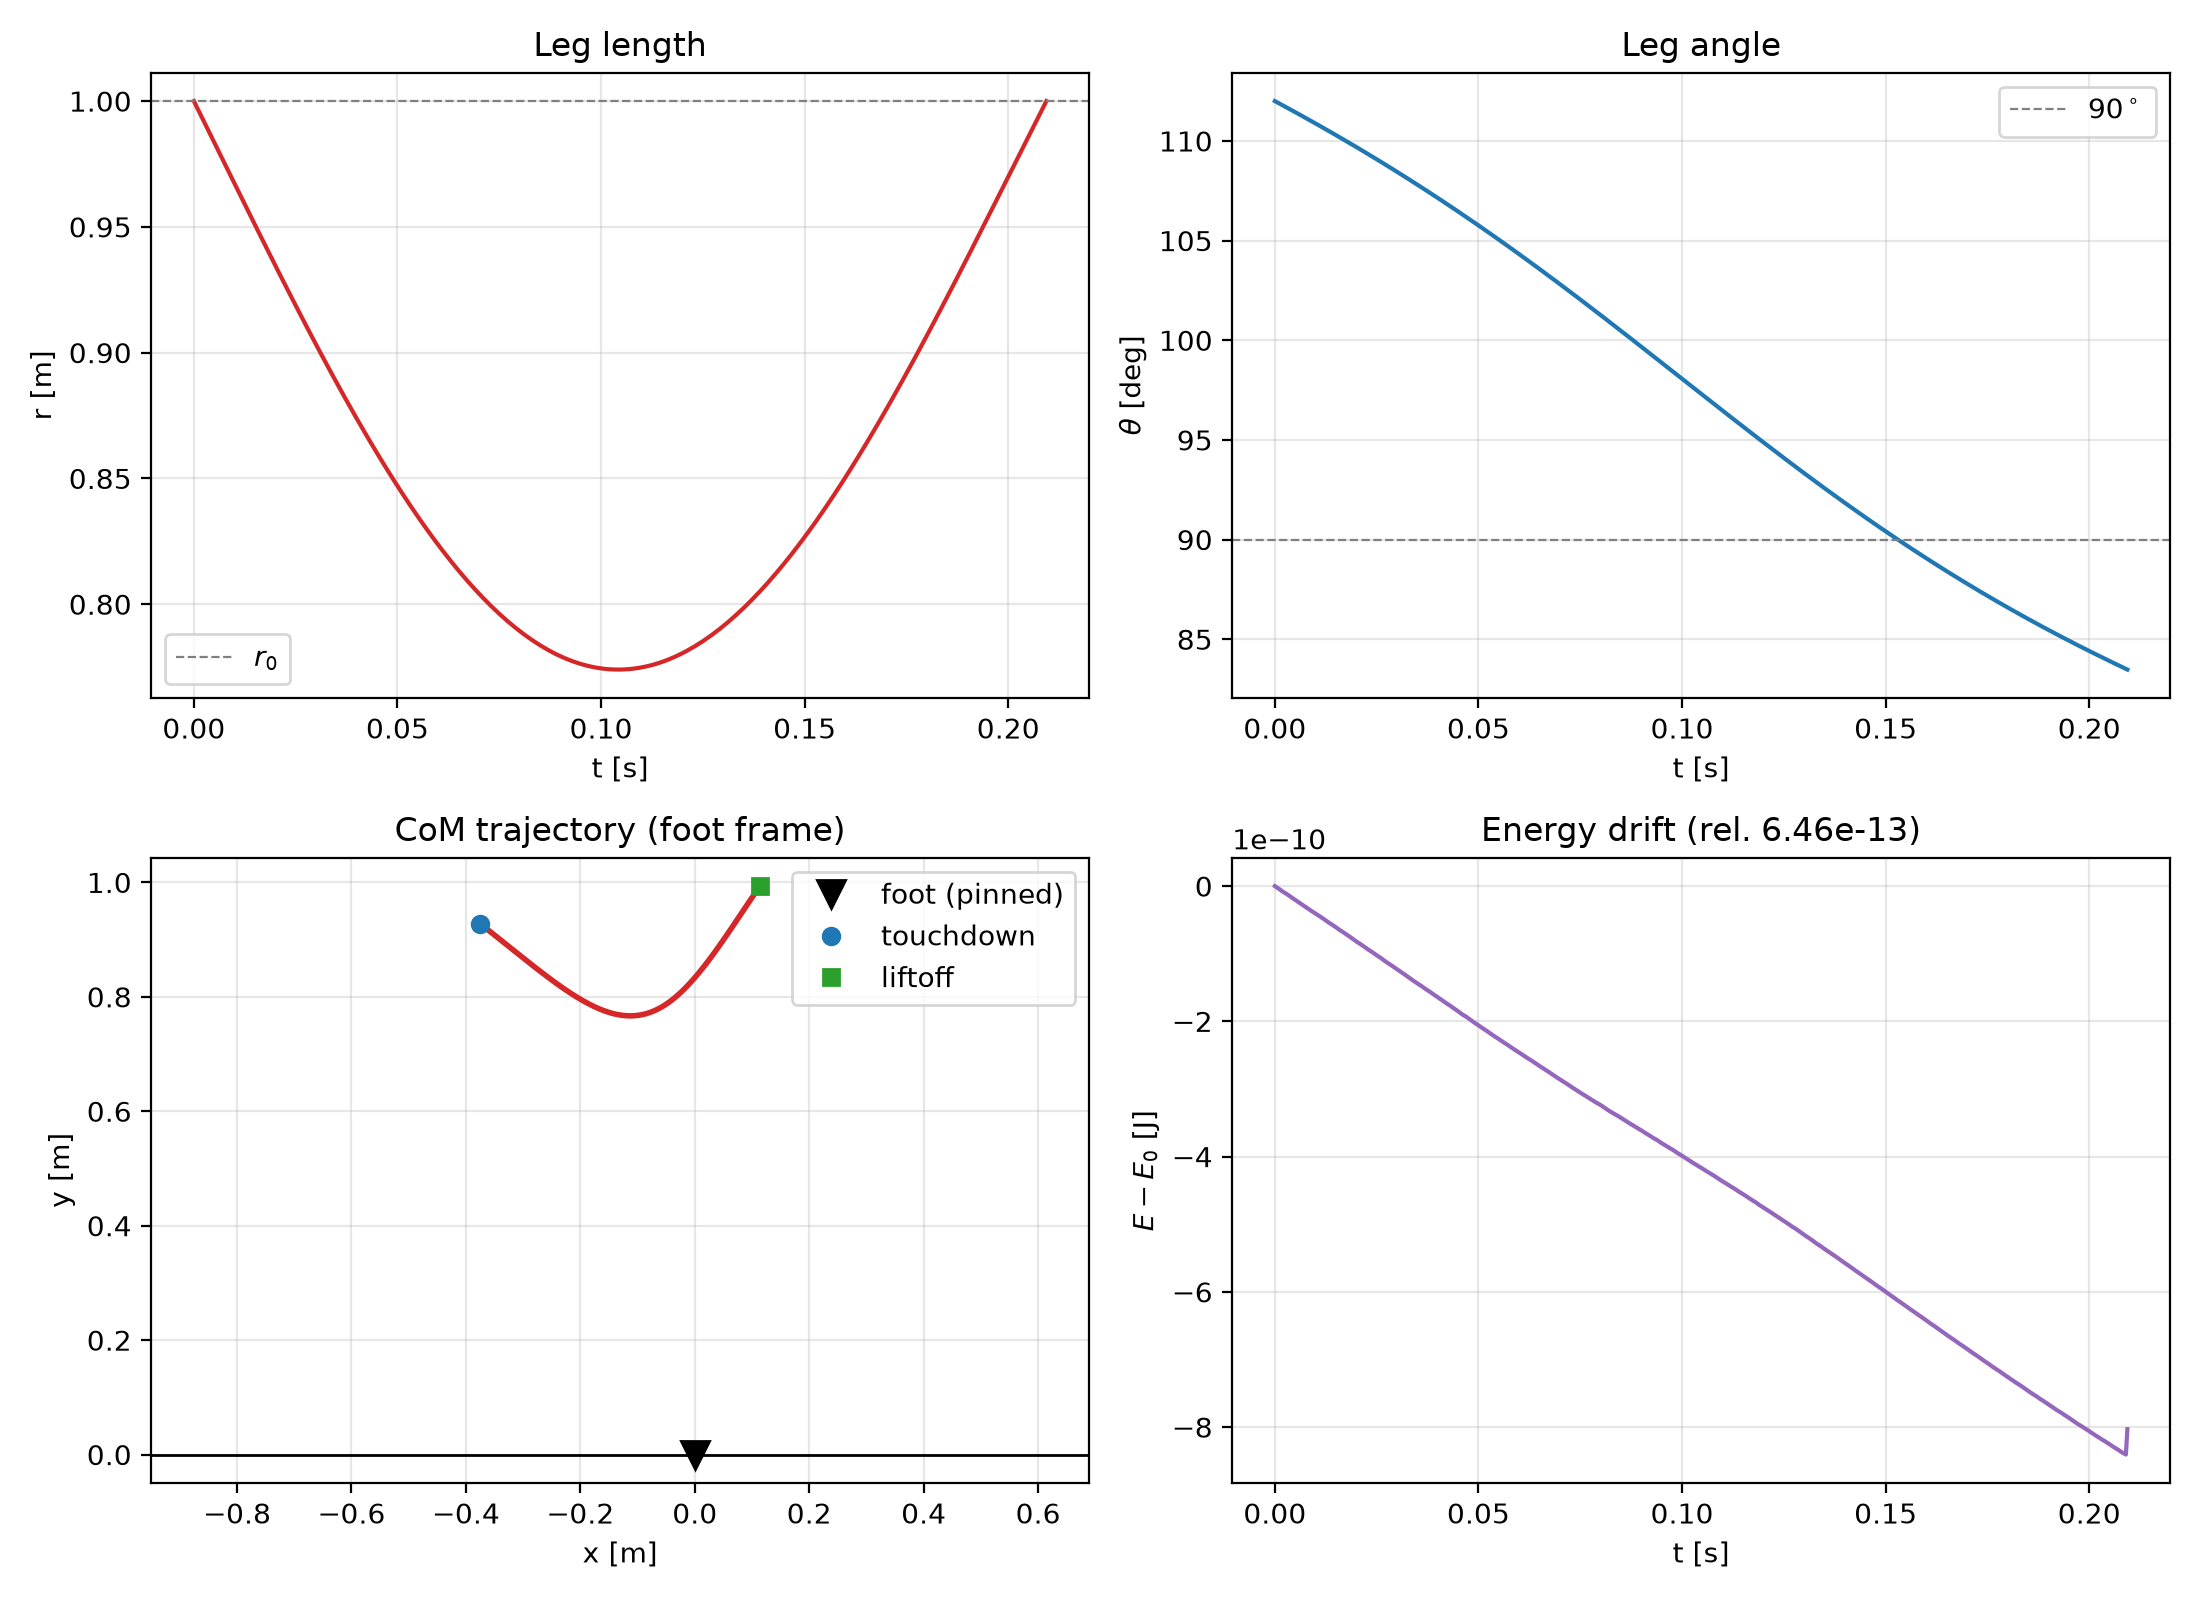
\includegraphics[width=0.85\linewidth]{Figures/Graphs/stance_validation.png}
    \caption{\footnotesize Stance simulation: $r(t)$, $\theta(t)$ (top),
    CoM trajectory (bottom left), energy drift (bottom right).}
    \label{fig:stance}
\end{figure}

\subsection{Full-Cycle Energy Conservation and Dimension-Reduction Validation}
\texttt{proveX\_dotIsRedundant()} validates the full hop cycle: starting
from the apex state of Section~4.1, it computes the apex energy $E_1$
(\texttt{energyHop()}), chains one hop -- flight $\to$ touchdown $\to$
stance $\to$ liftoff $\to$ flight (\texttt{hop()}) -- and recomputes
the apex energy $E_2$. Relative drift over the full cycle,
\[
    \frac{|E_2-E_1|}{|E_1|} = 6.17\times10^{-13},
\]
is consistent with the stance-only drift of Section~4.1
($6.46\times10^{-13}$), confirming total mechanical energy is
conserved across the full switching cycle, not just within stance.

The same run checks the dimension reduction of Section~2.7: with
$E_1$ fixed, $\dot x=\sqrt{2E_1/m-2gy}$ evaluated at the simulated
output height $y_{n+1}=1.4465$ m predicts $\dot x_{pred}=2.0403$ m/s,
matching the simulator's own $v_{x,n+1}=2.0403$ m/s to
\[
    \frac{|v_{x,n+1}-\dot x_{pred}|}{|\dot x_{pred}|} = 2.41\times10^{-12}.
\]

\subsection{Apex Return Map: Root-Finding Methodology and Result}
\label{sec:apexmapresult}
\texttt{findApexMapFixedPoint()} locates the root of $f(y)=P(y)-y$
(Section~2.8) over the domain of $y$ physically valid for a given
$(k,\theta_{TD},E)$: bounded below by the minimum apex height
consistent with touchdown at angle $\theta_{TD}$,
\[
    y_{min} = r_0\sin\theta_{TD},
\]
and above by the height at which the closed-form $\dot x$ of
Section~2.7 would require a negative value under the square root,
\[
    y_{max}=\frac{E}{mg}.
\]
A small inward padding ($\epsilon=10^{-3}$ m) is added to $y_{min}$
to avoid floating-point roundoff pushing the touchdown free-fall
relation's square root slightly negative at the exact boundary.

$f(y)$ is sampled coarsely (30 points) across $[y_{min},y_{max}]$;
once a bracket with a sign change is found, Brent's method refines it
to a root $y^\ast$, and $P'(y^\ast)$ is estimated by the central
difference of Section~2.8 with $dy=10^{-3}$ m.

For the validated parameter set of Section~4.1 ($m=80$ kg, $r_0=1$ m,
$k=20000$ N/m, $\theta_{TD}=68^\circ$, $E$ fixed by $y_0=1.2$ m,
$v_{x0}=3.0$ m/s):
\begin{result}
\[
    y^\ast \approx 1.5096\text{ m}, \qquad P'(y^\ast) \approx -2.76
\]
\end{result}
$|P'(y^\ast)|>1$: this fixed point is unstable, and the negative sign
indicates oscillatory divergence -- a perturbed apex height overshoots
on alternating sides of $y^\ast$, growing each hop. Steady hopping at
$\theta_{TD}=68^\circ$, $k=20000$ N/m is therefore not stable.

\subsection{Grid Sweep Methodology and Parameter Sweep}
\texttt{gridSearchFixedPoints()} wraps the pipeline of Section~4.3
into a function of $(k,\theta_{TD})$ returning $(y^\ast,P'(y^\ast))$,
or null if $f(y)$ has no sign change -- i.e.\ no periodic gait exists
there at this $E$. Each cell uses its own copy of the parameter
dictionary, so sweeping $k$ never mutates state shared across cells.
\texttt{stableBandWidth()} additionally reports the longest run of
contiguous stable cells along each grid direction, used below to tell
a genuinely narrow stability margin from a coarse-grid artifact.

An initial coarse $40\times40$ diagnostic grid over
$k\in[5000,40000]$ N/m, $\theta_{TD}\in[55^\circ,80^\circ]$ turned up
only a one-cell-wide staircase of stable cells (band width 2 cells
along $\theta_{TD}$, 3 along $k$) through an otherwise unstable field
-- too thin to trust at that resolution. \texttt{localRefinementSweep()}
zoomed a $20\times20$ window ($\pm2.5^\circ\times\pm2500$ N/m, roughly
$4\times$ finer) onto a representative stable cell near
$k\approx20256$ N/m, $\theta_{TD}\approx71.0^\circ$; there the band
\emph{thickened} (3 cells along $\theta_{TD}$, 5 along $k$), meaning
the coarse staircase was a grid-resolution artifact, so the full
sweep needed that finer spacing to be trustworthy.

The final grid matches that resolution across the whole domain: a
$133\times95$ sweep ($k\in[5000,40000]$ N/m in steps of
$\approx265$ N/m, $\theta_{TD}\in[55^\circ,80^\circ]$ in steps of
$\approx0.27^\circ$; 12{,}635 cells, only 5 with no fixed point),
classified stable/unstable/no-fixed-point in
Figure~\ref{fig:stability_sweep}, with the friction-cone floor from
Section~\ref{sec:apexmapresult} ($\theta_{TD}\ge59^\circ$, $\mu=0.6$)
overlaid. The band widens slightly here (3 cells along $\theta_{TD}$,
8 along $k$) but is still only a few cells across. A second local
refinement at the same fine spacing (Figure~\ref{fig:stability_refinement}),
centered on the final grid's own representative stable cell
($k\approx20114$ N/m, $\theta_{TD}\approx70.96^\circ$,
$y^\ast\approx0.9496$ m, $P'(y^\ast)\approx0.348$), gives a band width
of 3 cells along $\theta_{TD}$ and 5 along $k$ -- the same order as
the full grid, so the earlier thickening has stopped: the self-stable
region is a real, if narrow, sliver of $(k,\theta_{TD})$ space at this
$E$, not a grid-spacing artifact.

\begin{figure}[H]
    \centering
    
\includegraphics[width=0.72\linewidth]{Figures/Graphs/stability_sweep.png}
    \caption{\footnotesize Self-stable running region over the full
    $133\times95$ $(k,\theta_{TD})$ grid at fixed $E$ (Section~4.1
    parameters). Green: stable fixed point ($|P'(y^\ast)|<1$); orange:
    unstable; gray: no fixed point found. Dashed line/shading: the
    friction-cone floor $\theta_{TD}\ge59^\circ$ ($\mu=0.6$).}
    \label{fig:stability_sweep}
\end{figure}

\begin{figure}[H]
    \centering
    
\includegraphics[width=0.62\linewidth]{Figures/Graphs/stability_refinement.png}
    \caption{\footnotesize Local refinement ($20\times20$,
    $\pm2.5^\circ\times\pm2500$ N/m) around the stable band near
    $k\approx20114$ N/m, $\theta_{TD}\approx70.96^\circ$, at the same
    fine spacing used to validate Figure~\ref{fig:stability_sweep}'s
    resolution. The band's width here matches the full grid, confirming
    it is not still thickening.}
    \label{fig:stability_refinement}
\end{figure}

\subsection{Apex-Map Iteration: Cobweb Diagrams for the Stable and Unstable Cases}
\label{sec:cobweb}
Section~\ref{sec:apexmapresult} and Section~4.4 each report a fixed point and
a slope, but neither shows what convergence or divergence looks like hop to
hop. \texttt{plotApexMapIteration()} does that directly by iterating
$y_{n+1}=P(y_n)$ from a perturbed initial height and
plotting both the cobweb diagram (the map $P(y)$, the diagonal
$y_{n+1}=y_n$, and the resulting staircase) and $y_n$ vs.\ hop index $n$, for
two cases at the same fixed energy $E$: the stable representative cell of
Section~4.4 ($k\approx20114$ N/m, $\theta_{TD}\approx70.96^\circ$,
$y^\ast\approx0.9496$ m, $P'(y^\ast)\approx0.35$) and the unstable validated
point of Section~\ref{sec:apexmapresult} ($k=20000$ N/m, $\theta_{TD}=68^\circ$,
$y^\ast\approx1.5096$ m, $P'(y^\ast)\approx-2.76$).

Figure~\ref{fig:apex_iteration} confirms the qualitative prediction of
Section~2.8 from the sign and magnitude of $P'(y^\ast)$ alone: perturbing the
stable case by $+0.05$ m produces a monotonic staircase that steps down the
same side of the diagonal every hop, converging smoothly onto $y^\ast$. This
monotonic decay only shows up for a \emph{small} perturbation, which is
itself informative: the sweep only certifies \emph{local} stability, and a
larger perturbation instead wanders through the map's global nonlinearity
(the hump shape of $P(y)$ visible in the figure) before it happens to land
back near $y^\ast$, if it does at all. Perturbing the unstable case by only
$+0.02$ m, by contrast, produces a staircase that immediately crosses to the
other side of the diagonal every hop and spirals outward, consistent with
the oscillatory divergence already reported in Section~\ref{sec:apexmapresult}.

\begin{figure}[H]
    \centering
    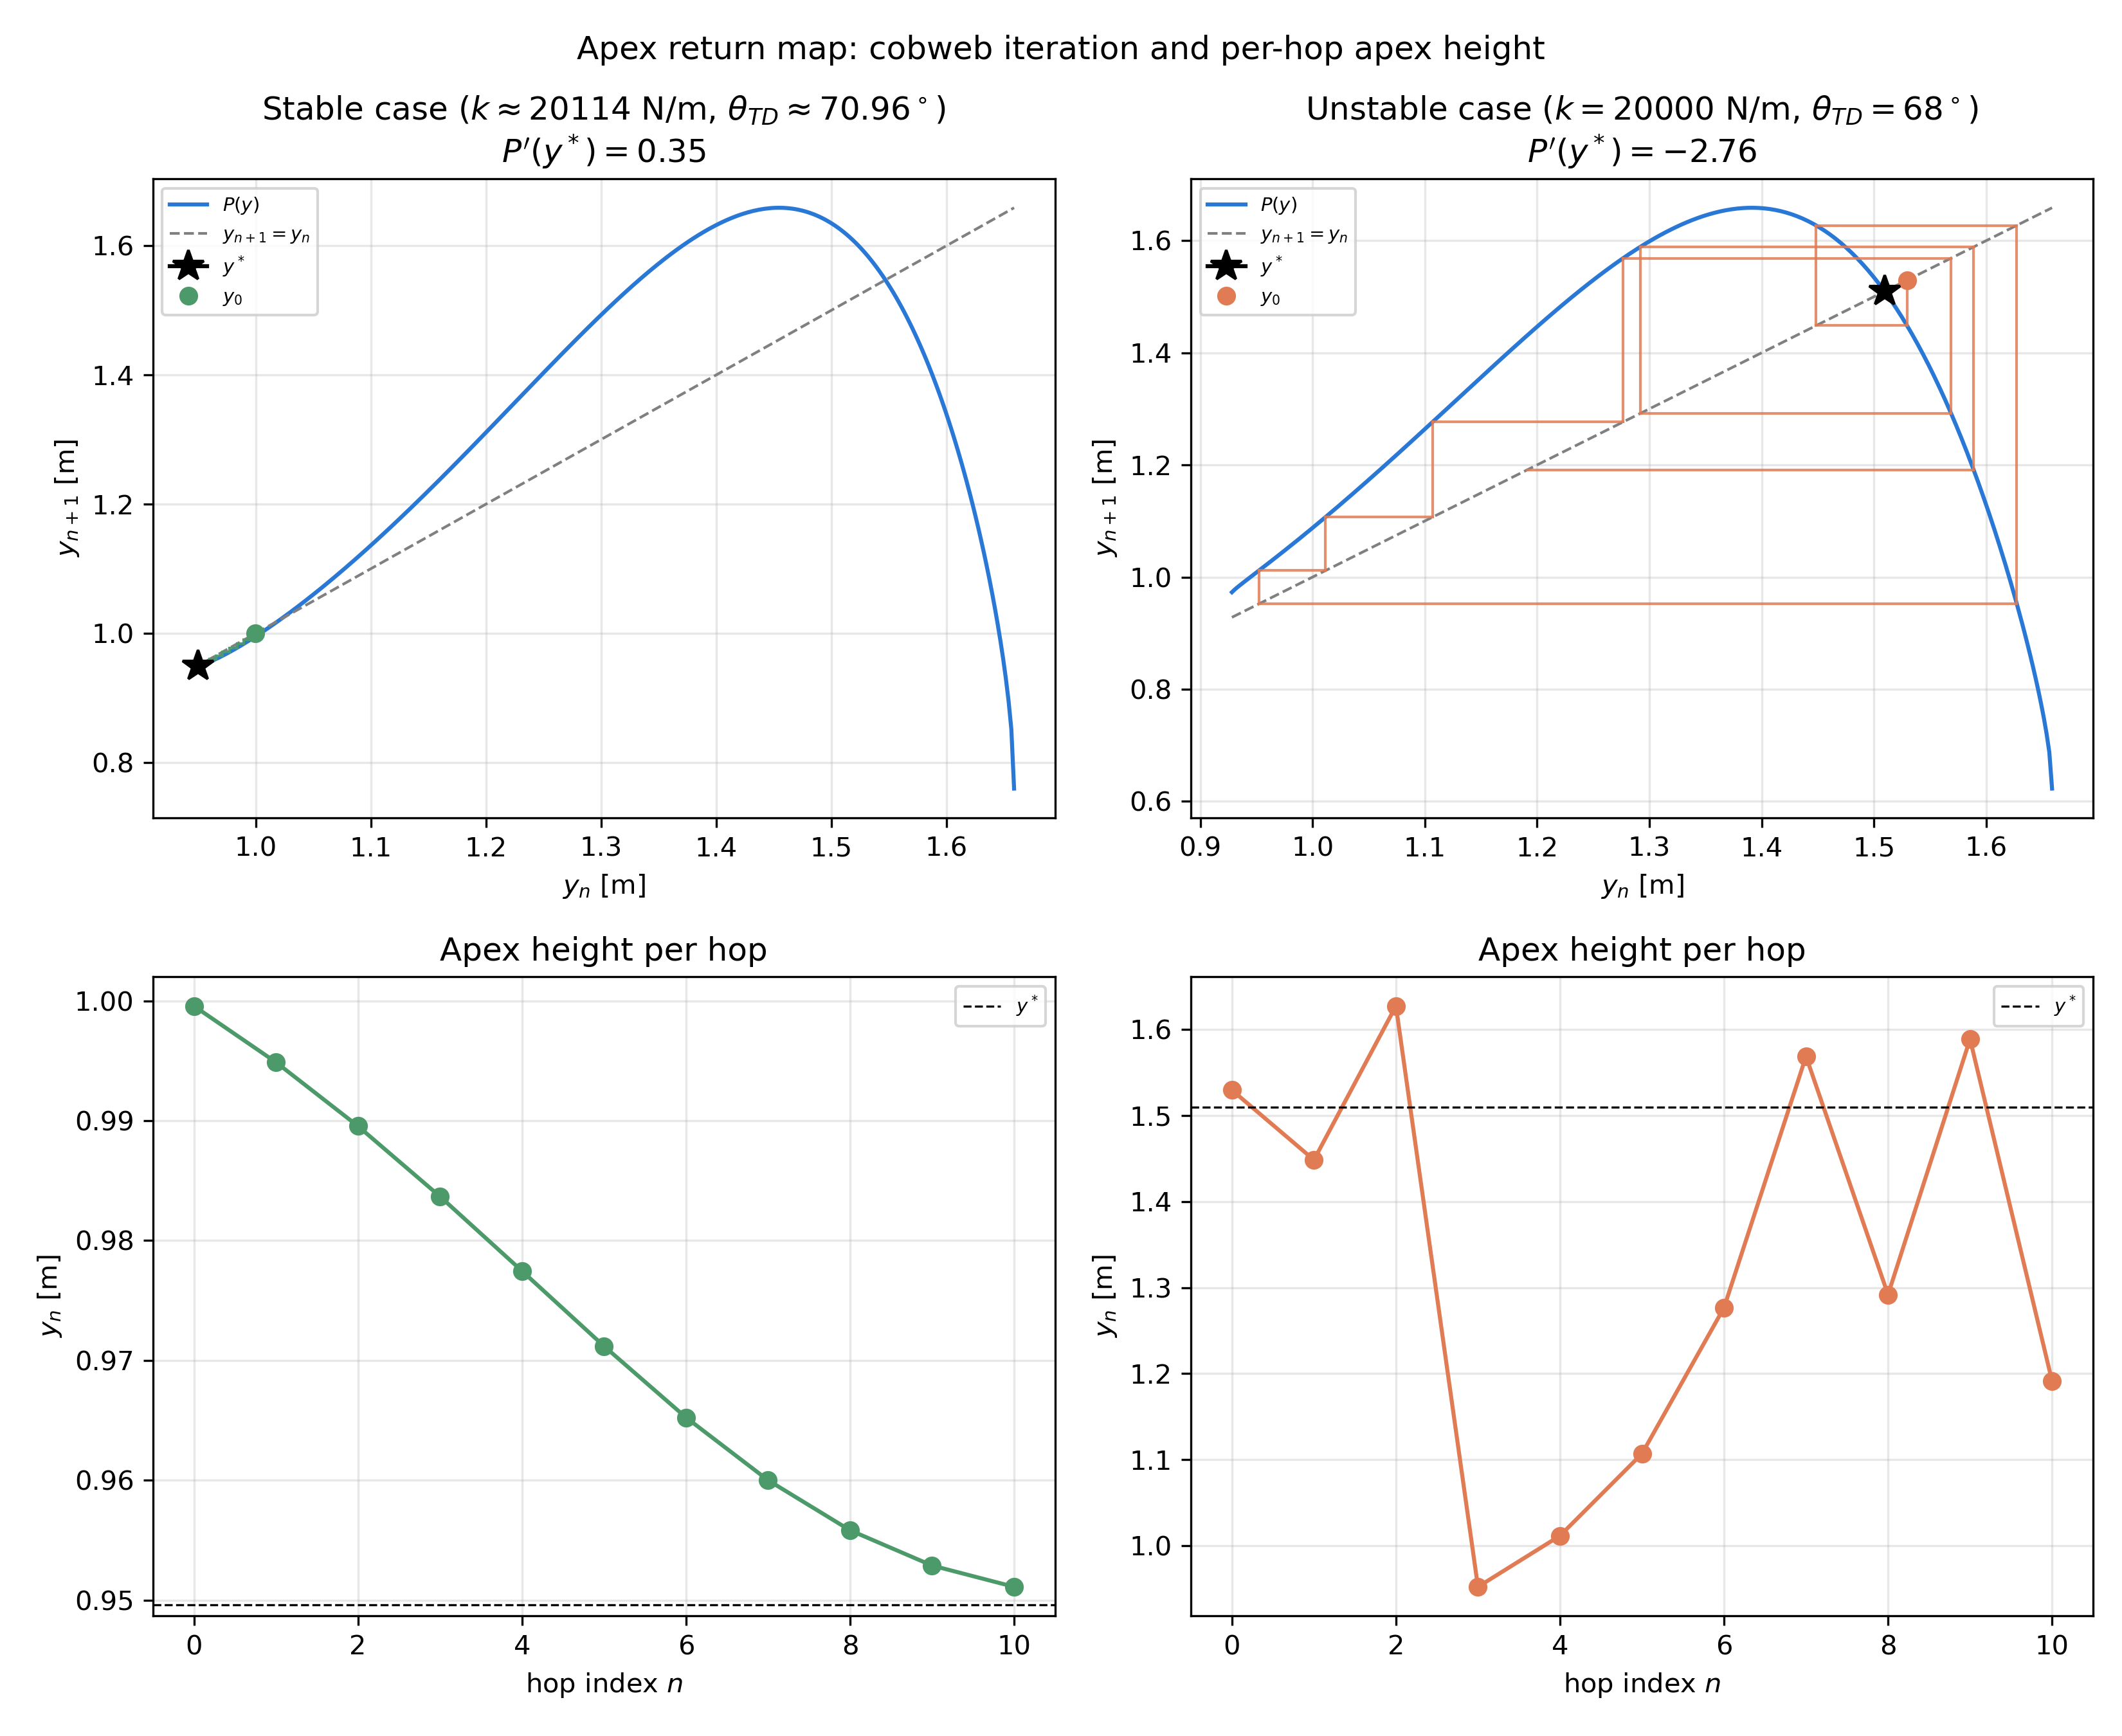
\includegraphics[width=0.95\linewidth]{Figures/Graphs/apex_map_iteration.png}
    \caption{\footnotesize Apex-map cobweb iteration (top) and apex height
    per hop (bottom) for the stable cell of Section~4.4 (left, green) and the
    unstable point of Section~\ref{sec:apexmapresult} (right, orange). The
    stable case converges monotonically for a small perturbation; the
    unstable case diverges, alternating sides of $y^\ast$ each hop.}
    \label{fig:apex_iteration}
\end{figure}

\subsection{Bifurcation Diagrams Along Each Sweep Direction}
\label{sec:bifurcation}
Section~4.4's grid already classifies every $(k,\theta_{TD})$ cell as
stable/unstable/no-fixed-point, but a single 2-D classification map does not
show \emph{how} the fixed point loses stability as a parameter varies
continuously. \texttt{plotBifurcationDiagrams()} slices two 1-D bifurcation
diagrams out of that same grid, both through the representative stable cell:
$y^\ast$ and $P'(y^\ast)$ vs.\ $\theta_{TD}$ at fixed $k\approx20114$ N/m,
and vs.\ $k$ at fixed $\theta_{TD}\approx70.96^\circ$
(Figure~\ref{fig:bifurcation}).

Both slices show the same structure: $y^\ast(\theta_{TD})$ and $y^\ast(k)$
vary smoothly and almost linearly, with no branching or discontinuity, so
this is not a classical saddle-node or pitchfork bifurcation in $y^\ast$.
Instead the loss of stability lives entirely in $P'(y^\ast)$: it crosses
$+1$ sharply at both edges of the narrow stable window (the thin green band
already visible in Figure~\ref{fig:stability_sweep}), confirming that the
self-stable region is bounded by genuine $|P'(y^\ast)|=1$ crossings at both
edges of the band, not by a grid-resolution artifact.

\begin{figure}[H]
    \centering
    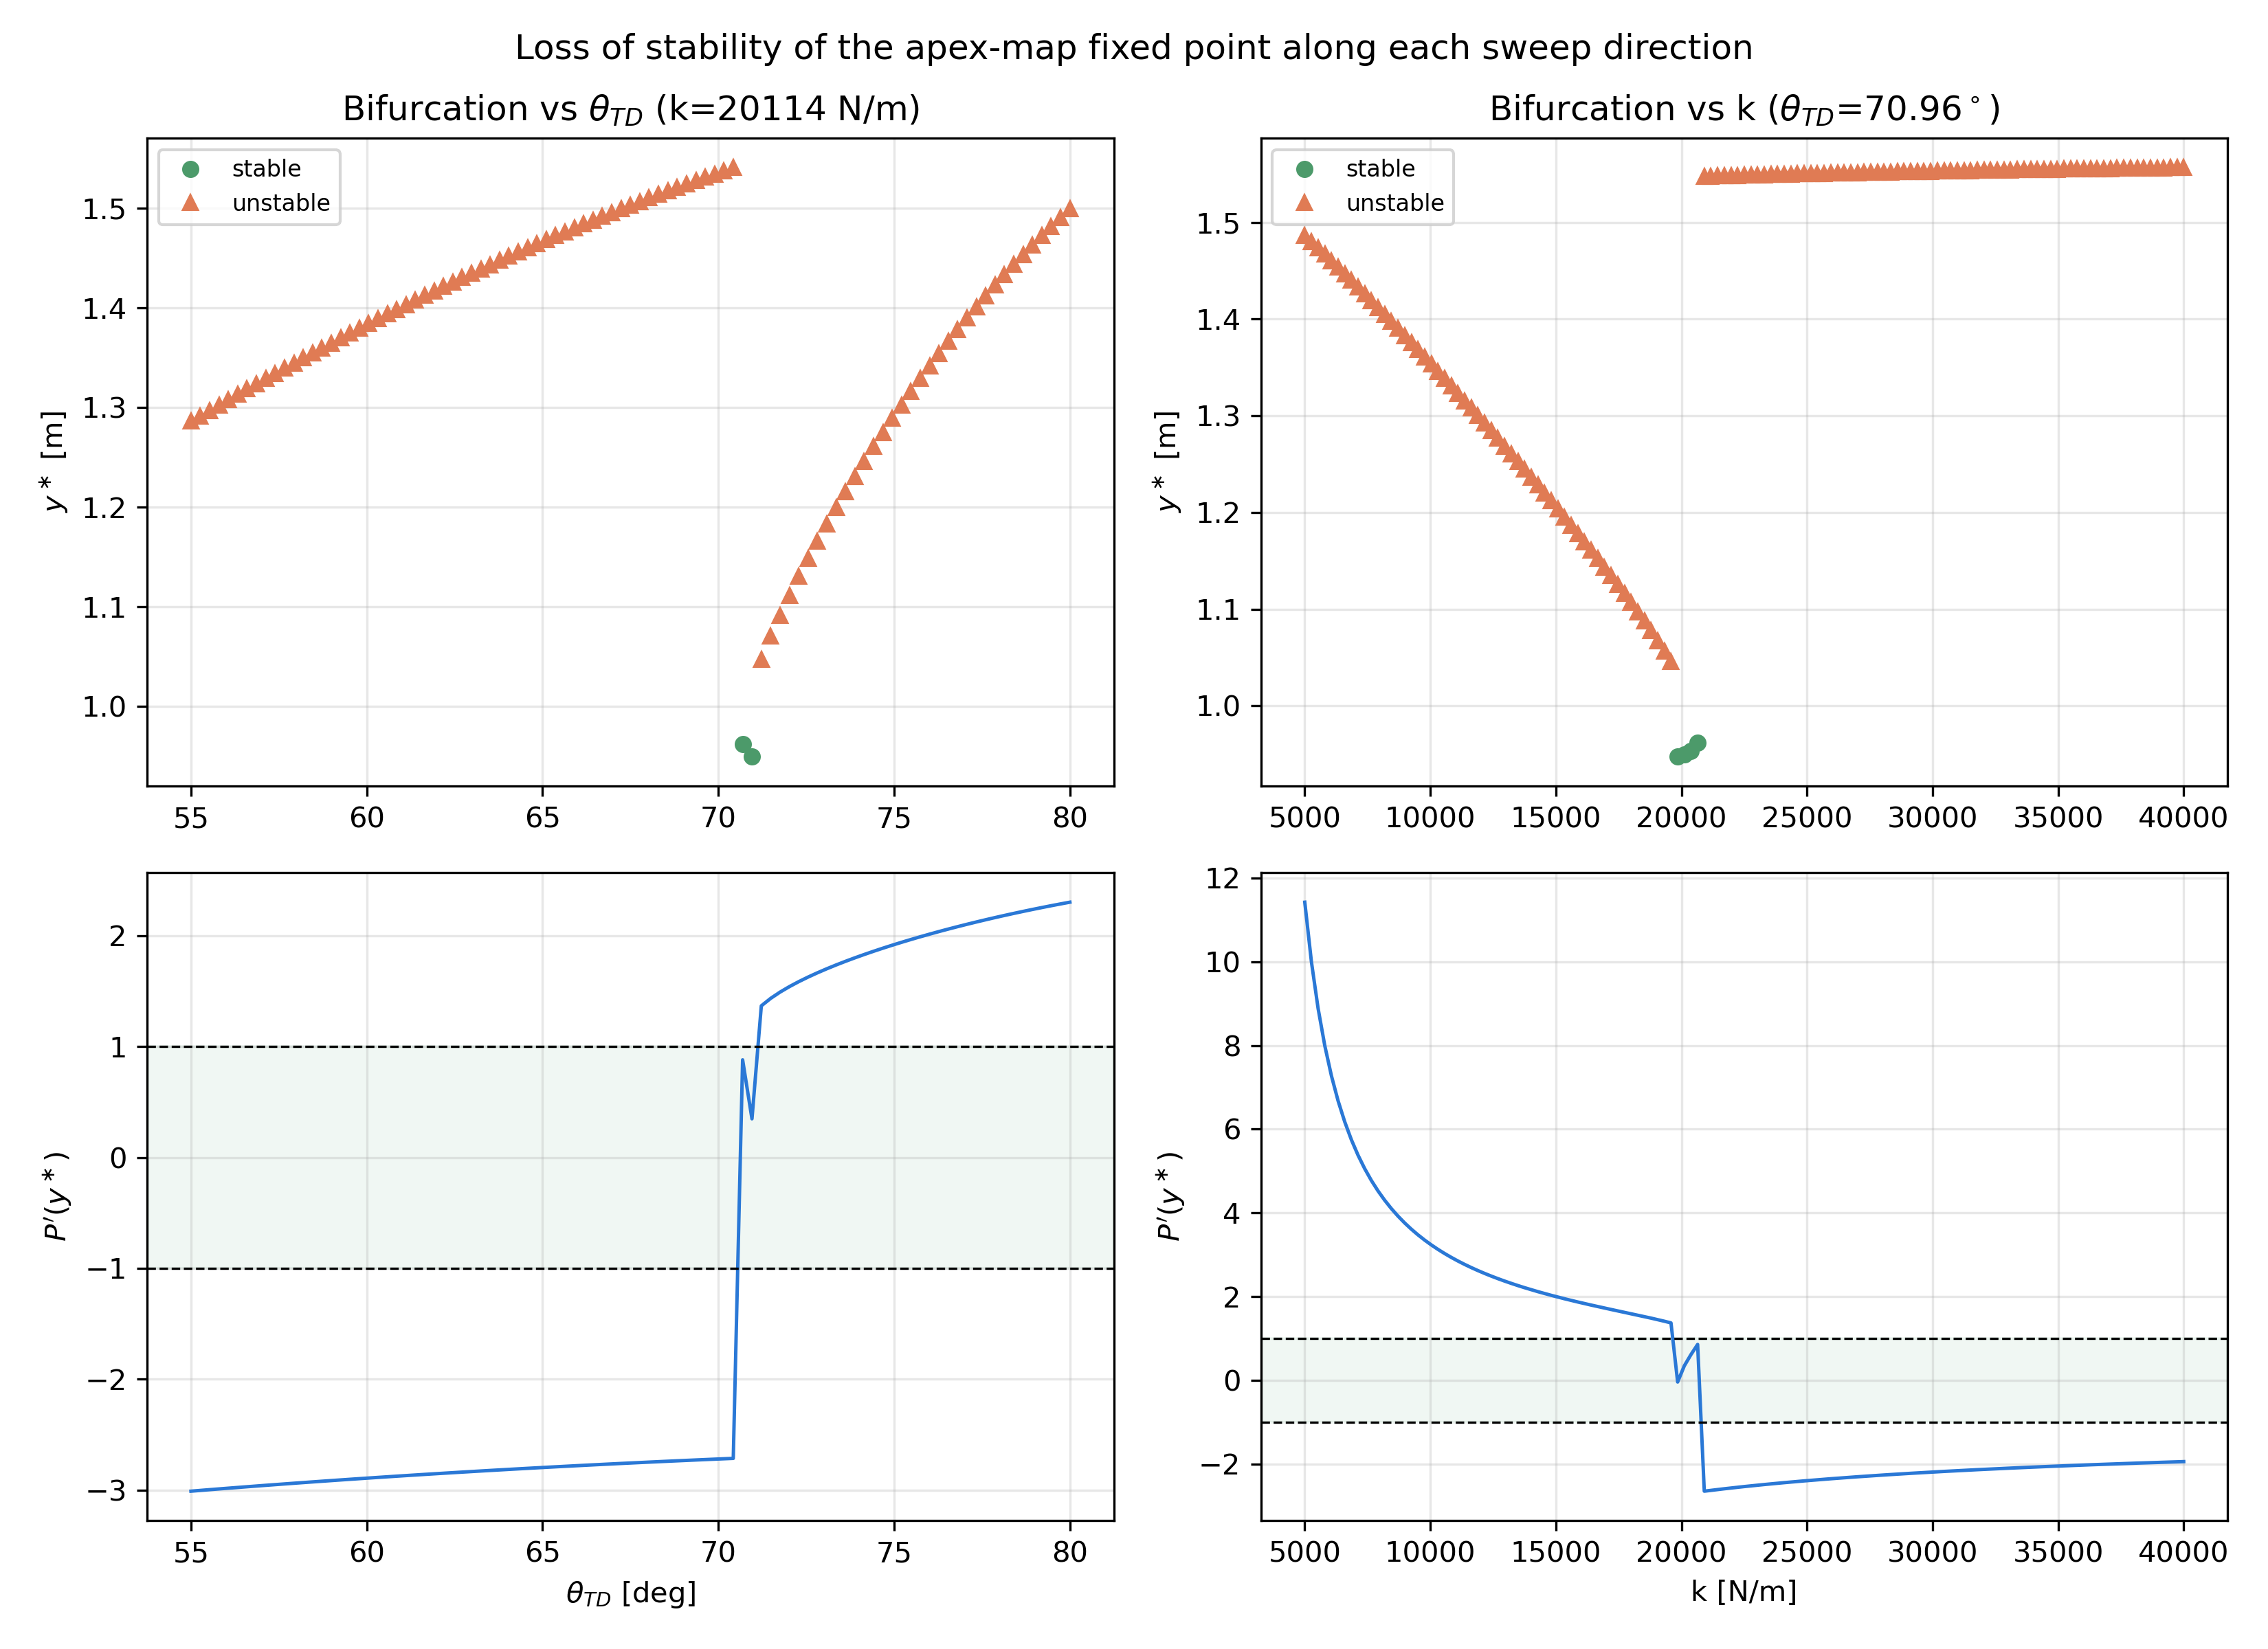
\includegraphics[width=0.95\linewidth]{Figures/Graphs/bifurcation_diagrams.png}
    \caption{\footnotesize Bifurcation diagrams: fixed-point height
    $y^\ast$ (top) and slope $P'(y^\ast)$ (bottom) vs.\ $\theta_{TD}$ at
    fixed $k$ (left) and vs.\ $k$ at fixed $\theta_{TD}$ (right), sliced
    through the representative stable cell of Section~4.4. Shaded band:
    $|P'(y^\ast)|<1$ (stable). Marker shape doubles the stable/unstable
    color coding.}
    \label{fig:bifurcation}
\end{figure}

\subsection{Stance-Phase Portrait}
\label{sec:phaseportrait}
Section~1 motivates SLIP as building on the elastic pendulum studied in
class. \texttt{stancePhasePortrait()} makes that connection concrete by
plotting the stance-phase trajectory in the $(r,\dot r)$ and
$(\theta,\dot\theta)$ phase planes for several touchdown angles at the same
fixed apex energy (Figure~\ref{fig:phase_portrait}). Each trajectory is an
open arc, not a closed orbit: stance is a single finite-time pass through
phase space between the touchdown event (circle) and the liftoff event
(square), not a free-running periodic oscillator -- $r=r_0$ at both
switching events, but $\dot r$ changes sign in between as the leg compresses
and rebounds. Steeper touchdown angles produce shorter, less compressed
arcs that stay close to $r=r_0$, consistent with a more vertical landing
imparting less compression, while shallower angles compress the leg
further and sweep through a wider range of $\theta$.

\begin{figure}[H]
    \centering
    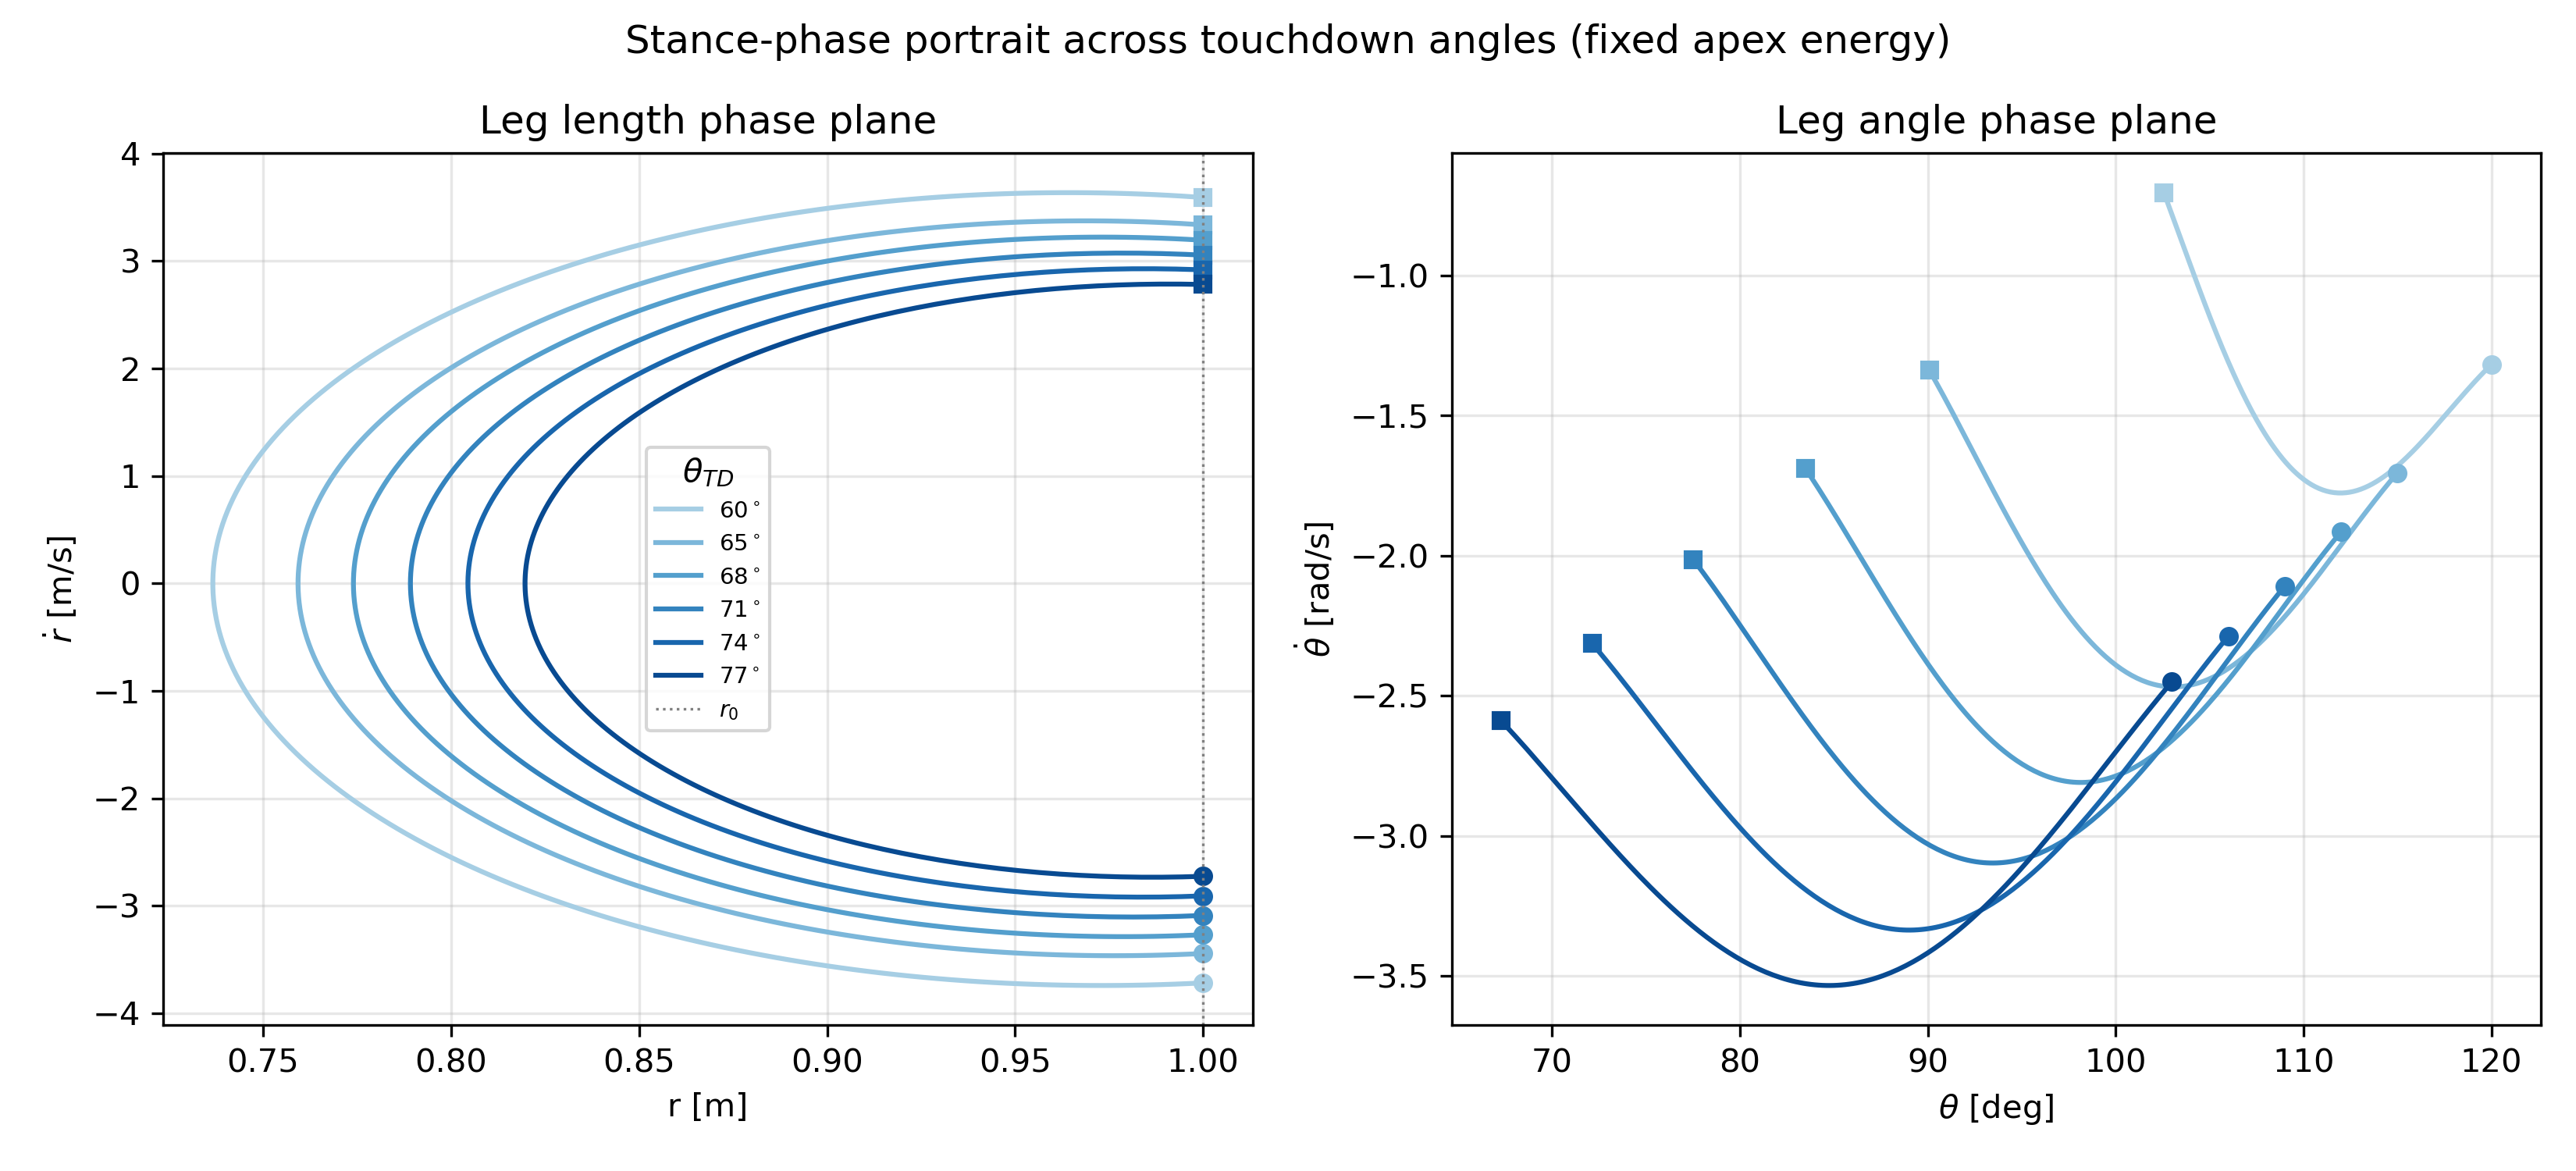
\includegraphics[width=0.95\linewidth]{Figures/Graphs/stance_phase_portrait.png}
    \caption{\footnotesize Stance-phase trajectories in the leg-length
    $(r,\dot r)$ and leg-angle $(\theta,\dot\theta)$ phase planes across
    touchdown angles $\theta_{TD}\in[60^\circ,77^\circ]$ at fixed apex
    energy. Circle = touchdown, square = liftoffStateSwitch.}
    \label{fig:phase_portrait}
\end{figure}

% ====================================================
% 5. LESSONS LEARNED
% ====================================================
\section{Lessons Learned}
This project was informative. It let me work through a multi-stage dynamic system and taught me how to handle state
transition conditions clearly. It also expanded on our study of geometric dynamics analysis by requiring a different
stability mechanism: instead of analyzing the whole system, we only need the points in space that best define the
motion. It also drove home that finding a periodic solution is not the same as finding a stable one: the fixed point
of the apex return map exists whether or not it is attracting, so stability has to be checked separately -- and for
the validated parameters, the hopping gait turned out not to be stable at all.

It was also a good project for working through robotics-style problems. The inverted pendulum is a famous model
throughout robotics, but with the Lagrangian this derivation becomes relatively simple, opening the door to more
accurate models. The parameter sweep also taught me a practical lesson about trusting numerical results: the first
coarse grid over $(k,\theta_{TD})$ turned up a stable band thin enough to be a grid-resolution artifact, and only
after refining the grid and confirming the band held its width could I be confident the narrow self-stable region
was a real feature of the model, not a numerical accident.



% ====================================================
% REFERENCES
% ====================================================
\newpage
\footnotesize
\begin{thebibliography}{9}
\setlength{\itemsep}{0pt}
\bibitem{blickhan1989}
R.~Blickhan, ``The spring-mass model for running and hopping,''
\textit{Journal of Biomechanics}, vol.~22, no.~11--12, pp.~1217--1227,
1989.
\bibitem{mcmahon1990}
T.~A.~McMahon and G.~C.~Cheng, ``The mechanics of running: how does
stiffness couple with speed?,'' \textit{Journal of Biomechanics},
vol.~23, suppl.~1, pp.~65--78, 1990.
\bibitem{full1999}
R.~J.~Full and D.~E.~Koditschek, ``Templates and anchors:
neuromechanical hypotheses of legged locomotion on land,''
\textit{Journal of Experimental Biology}, vol.~202, no.~23,
pp.~3325--3332, 1999.
\bibitem{schwind2000}
W.~J.~Schwind and D.~E.~Koditschek, ``Approximating the stance map of
a 2-DOF monoped runner,'' \textit{Journal of Nonlinear Science},
vol.~10, pp.~533--568, 2000.
\bibitem{saranli2001}
U.~Saranli, M.~Buehler, and D.~E.~Koditschek, ``RHex: a simple and
highly mobile hexapod robot,'' \textit{International Journal of
Robotics Research}, vol.~20, no.~7, pp.~616--631, 2001.
\bibitem{geyer2006}
H.~Geyer, A.~Seyfarth, and R.~Blickhan, ``Compliant leg behaviour
explains basic dynamics of walking and running,'' \textit{Proceedings
of the Royal Society B}, vol.~273, no.~1603, pp.~2861--2867, 2006.
\end{thebibliography}

% ====================================================
% APPENDIX
% ====================================================
\normalsize

\appendix
\section*{Appendix: Code}
\texttt{main.py} -- touchdown map, stance-phase RHS, and the
single-stance simulation and validation plots discussed in
Section~4.1.
\lstinputlisting[style=pystyle]{../Code/main.py}

\end{document}
